\documentclass{standalone}
\usepackage{graphicx}	
\usepackage{amssymb, amsmath}
\usepackage{color}

\usepackage{tikz}
\usetikzlibrary{intersections, backgrounds}
\usepackage{pgfmath}

\definecolor{light}{RGB}{220, 188, 188}
\definecolor{mid}{RGB}{185, 124, 124}
\definecolor{dark}{RGB}{143, 39, 39}
\definecolor{highlight}{RGB}{180, 31, 180}
\definecolor{gray10}{gray}{0.1}
\definecolor{gray20}{gray}{0.2}
\definecolor{gray30}{gray}{0.3}
\definecolor{gray40}{gray}{0.4}
\definecolor{gray60}{gray}{0.6}
\definecolor{gray70}{gray}{0.7}
\definecolor{gray80}{gray}{0.8}
\definecolor{gray90}{gray}{0.9}
\definecolor{gray95}{gray}{0.95}

\newcommand*{\offset}{0.025}

\begin{document}

\begin{tikzpicture}[scale=0.3, thick]

% Left
\begin{scope}[shift={(-36, 0)}]

\draw[white] (-17, 0) rectangle (17, 15);

\fill[dark] (-10, 4) circle (1);
\begin{scope}
  \clip (-10, 4) circle (1);
  \draw[color=light, line width=5, rotate=30] (-5.25, 8.25) arc[x radius=1.4, y radius=0.2, start angle=0, end angle=-180];
\end{scope}
\node at (-10, 10) {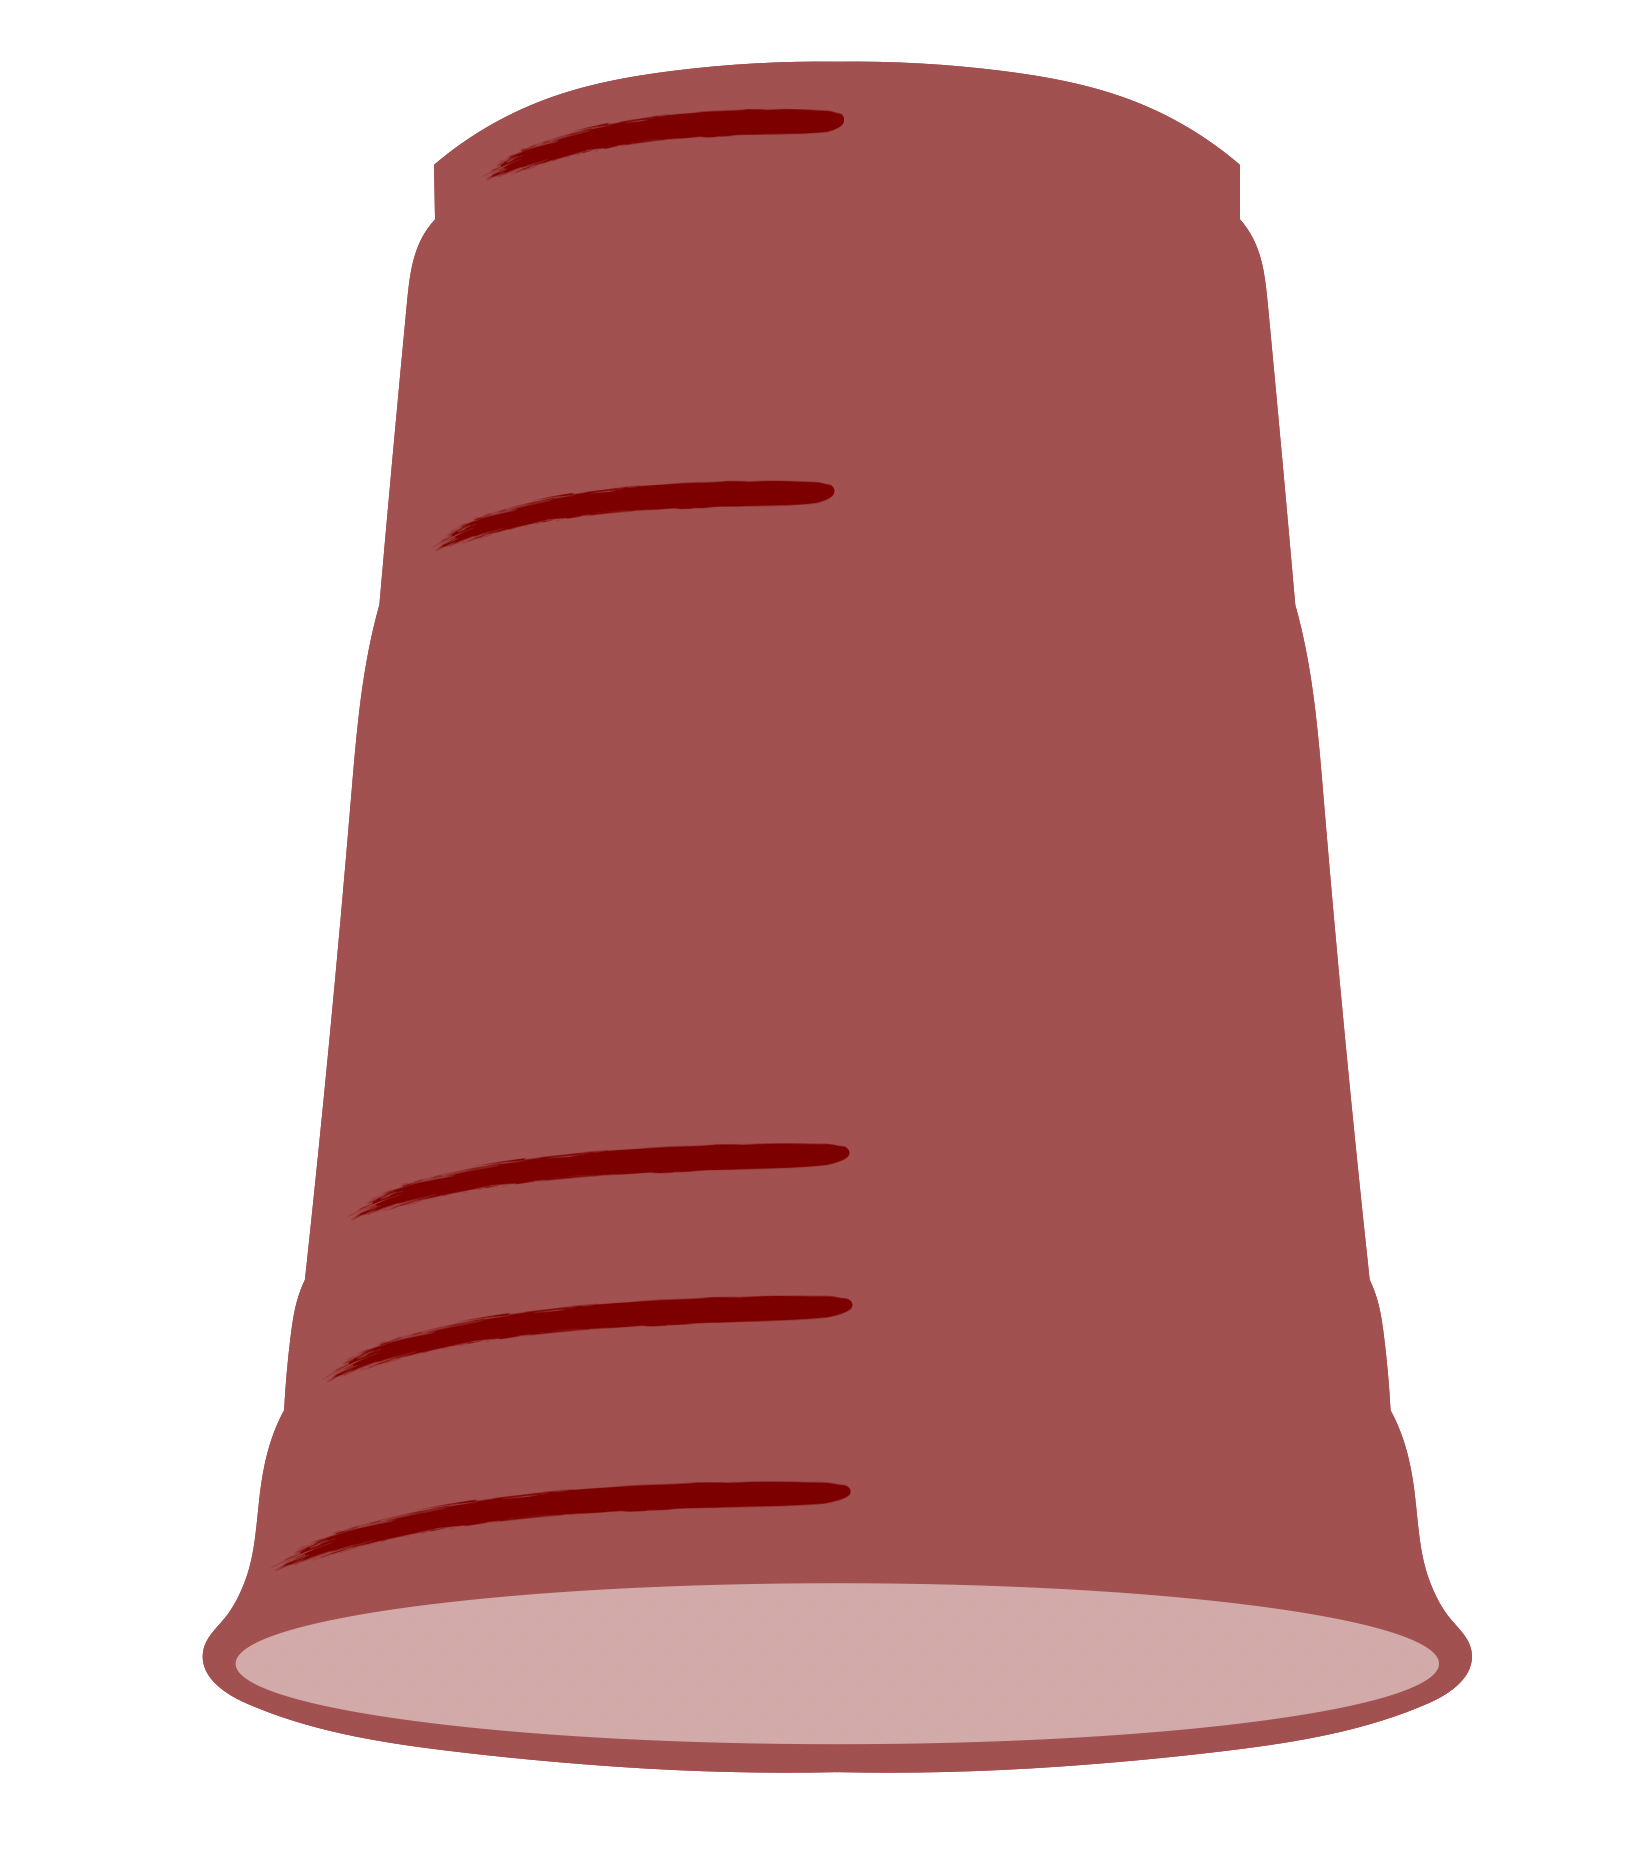
\includegraphics[width=2cm]{cup_up.png}};
  
\fill[mid] (0, 4) circle (1);
\begin{scope}
  \clip (0, 4) circle (1);
  \draw[color=dark, line width=2] (1.1, 4.3) arc[x radius=1.1, y radius=0.2, start angle=0, end angle=180];
  \draw[color=dark, line width=2] (1.1, 3.7) arc[x radius=1.1, y radius=0.2, start angle=0, end angle=180];
\end{scope}
\node at (0, 10) {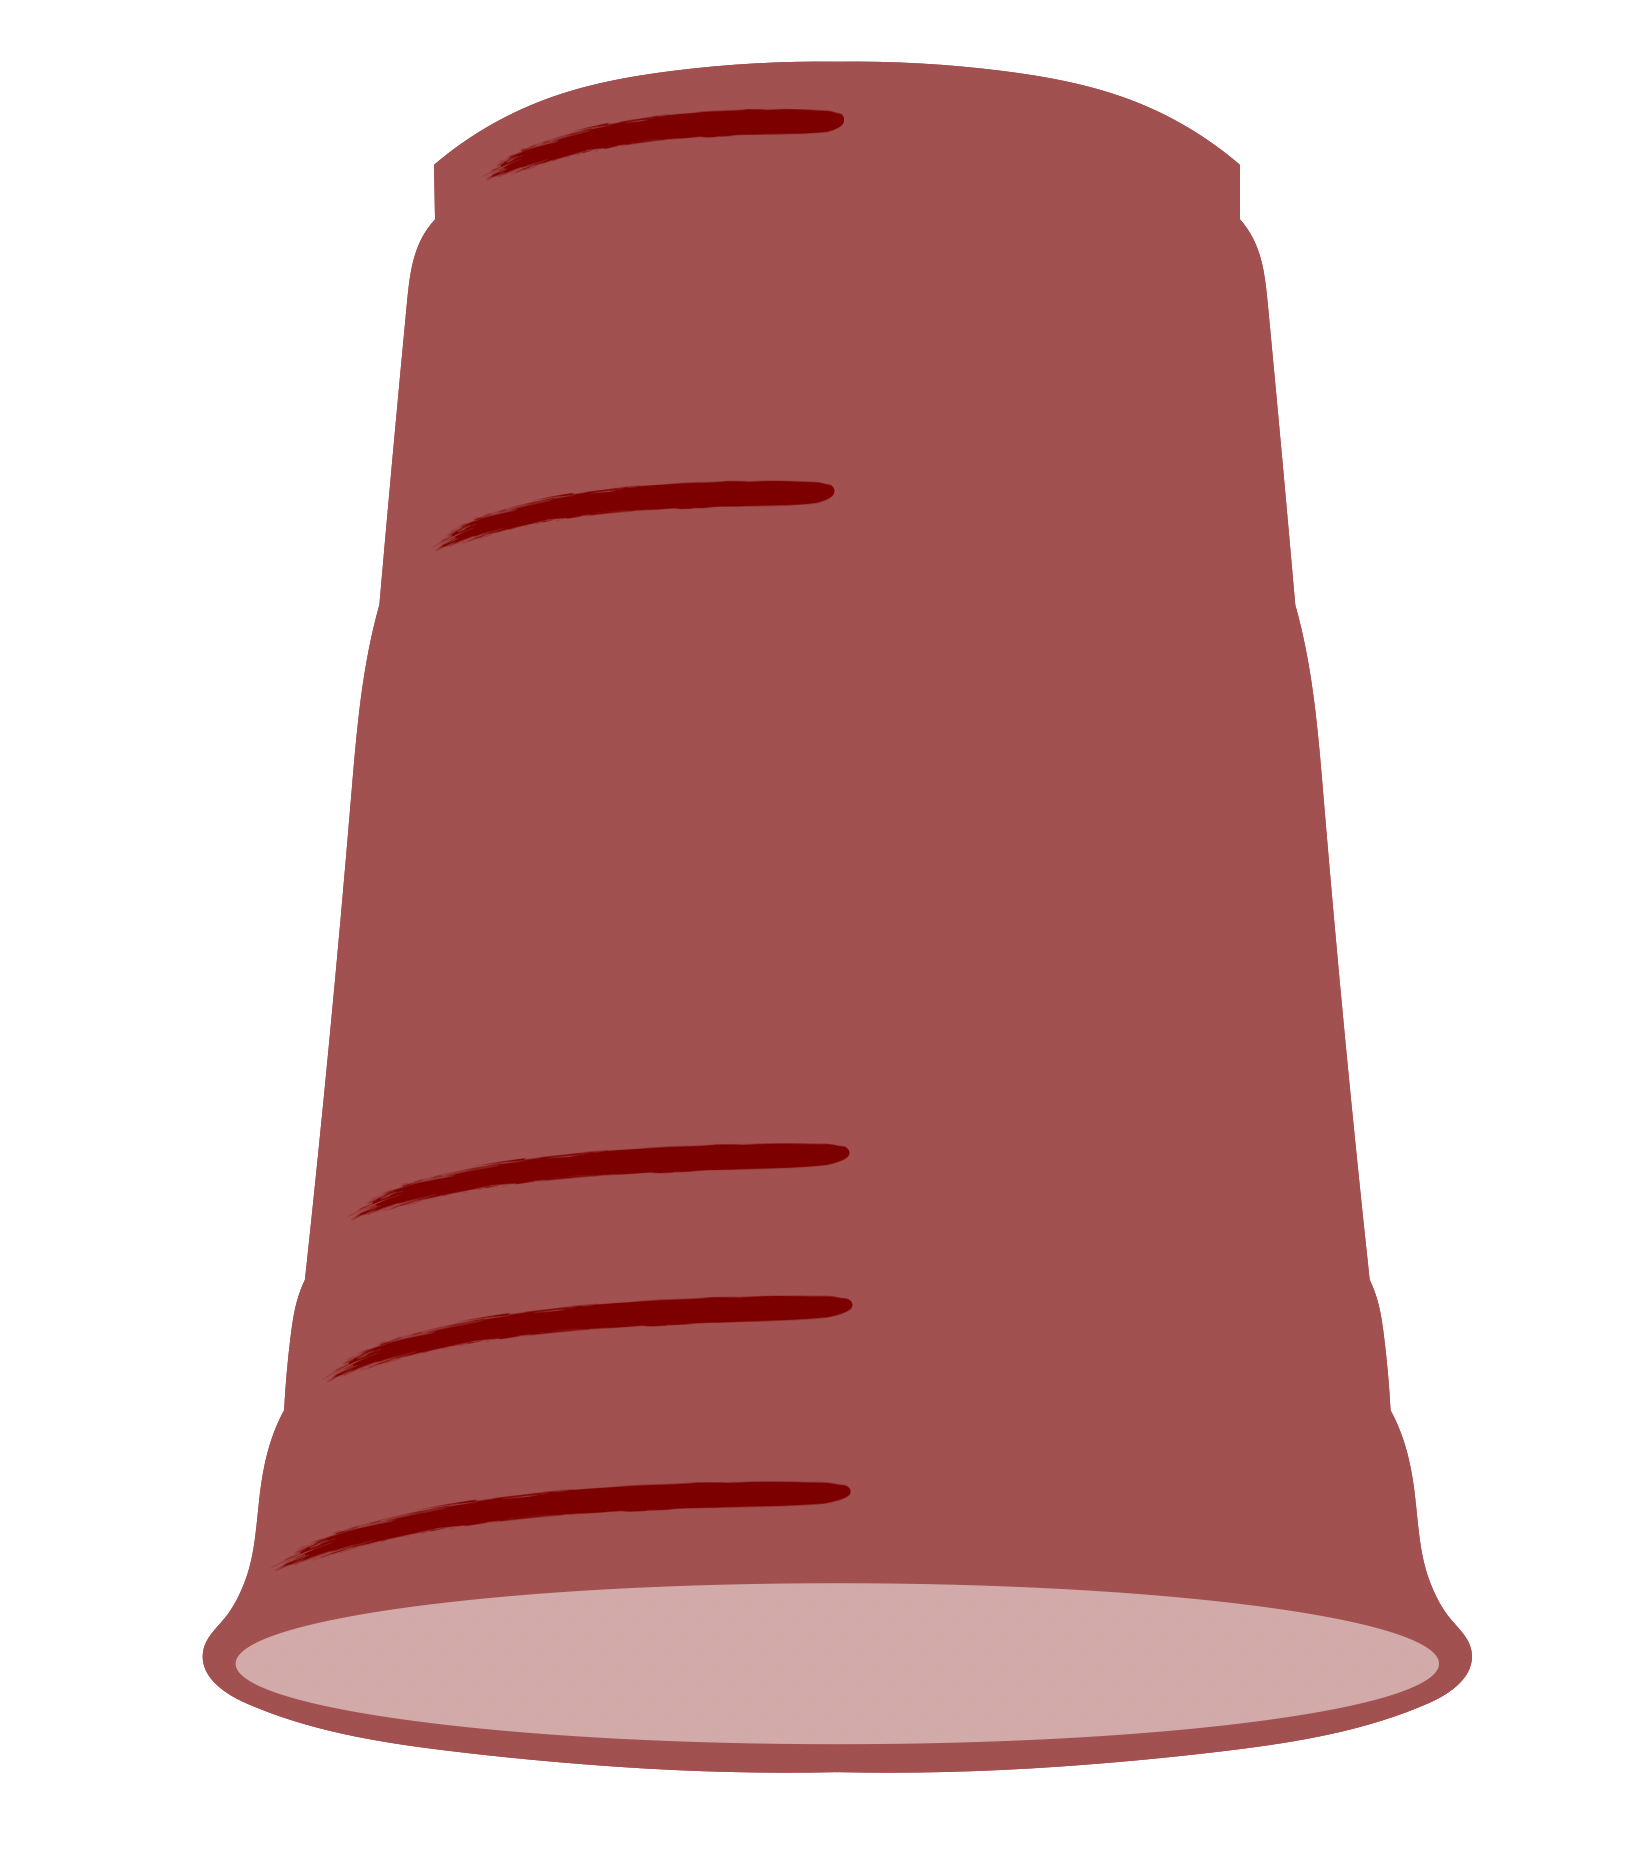
\includegraphics[width=2cm]{cup_up.png}};

\fill[dark] (+10, 4) circle (1);
\begin{scope}
  \clip (10, 4) circle (1);
  \draw[color=mid, line width=1] (10, 3) -- (10, 5);
  \draw[color=mid, line width=1] (10.25, 5) arc[x radius=0.3, y radius=1.1, start angle=90, end angle=-90];
  \draw[color=mid, line width=1] (9.75, 5) arc[x radius=0.3, y radius=1.1, start angle=90, end angle=270];
\end{scope}
\node at (+10, 10) {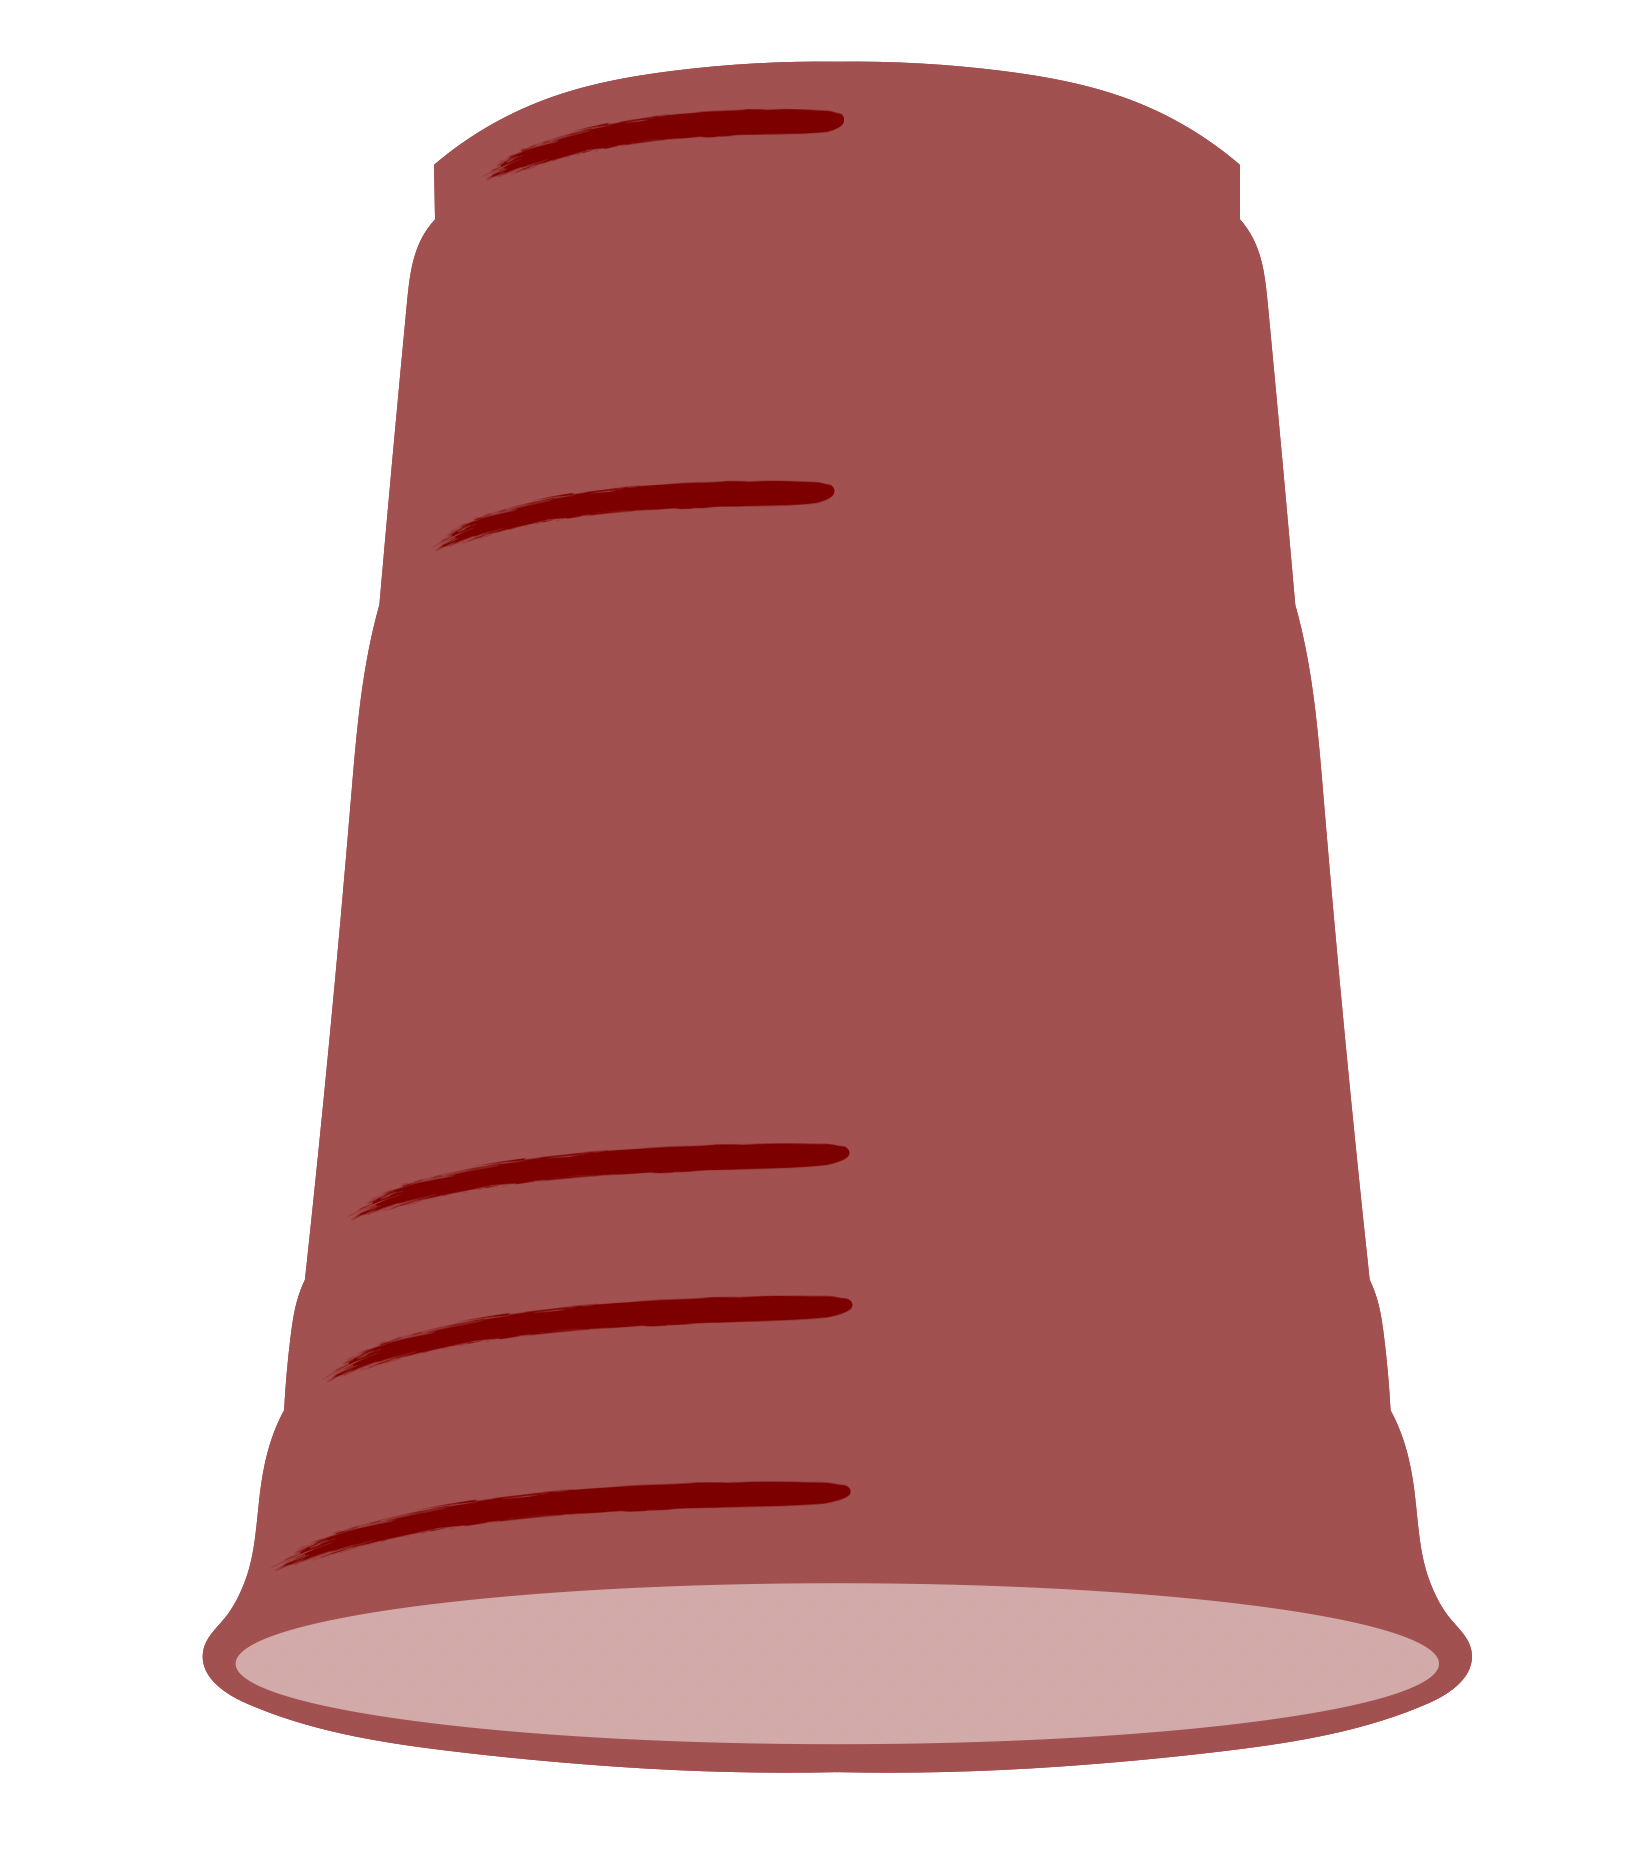
\includegraphics[width=2cm]{cup_up.png}};

\end{scope}

% Middle
\begin{scope}[shift={(0, 0)}]

\draw[white] (-17, 0) rectangle (17, 15);

\fill[dark] (-10, 4) circle (1);
\node at (-10, 7) {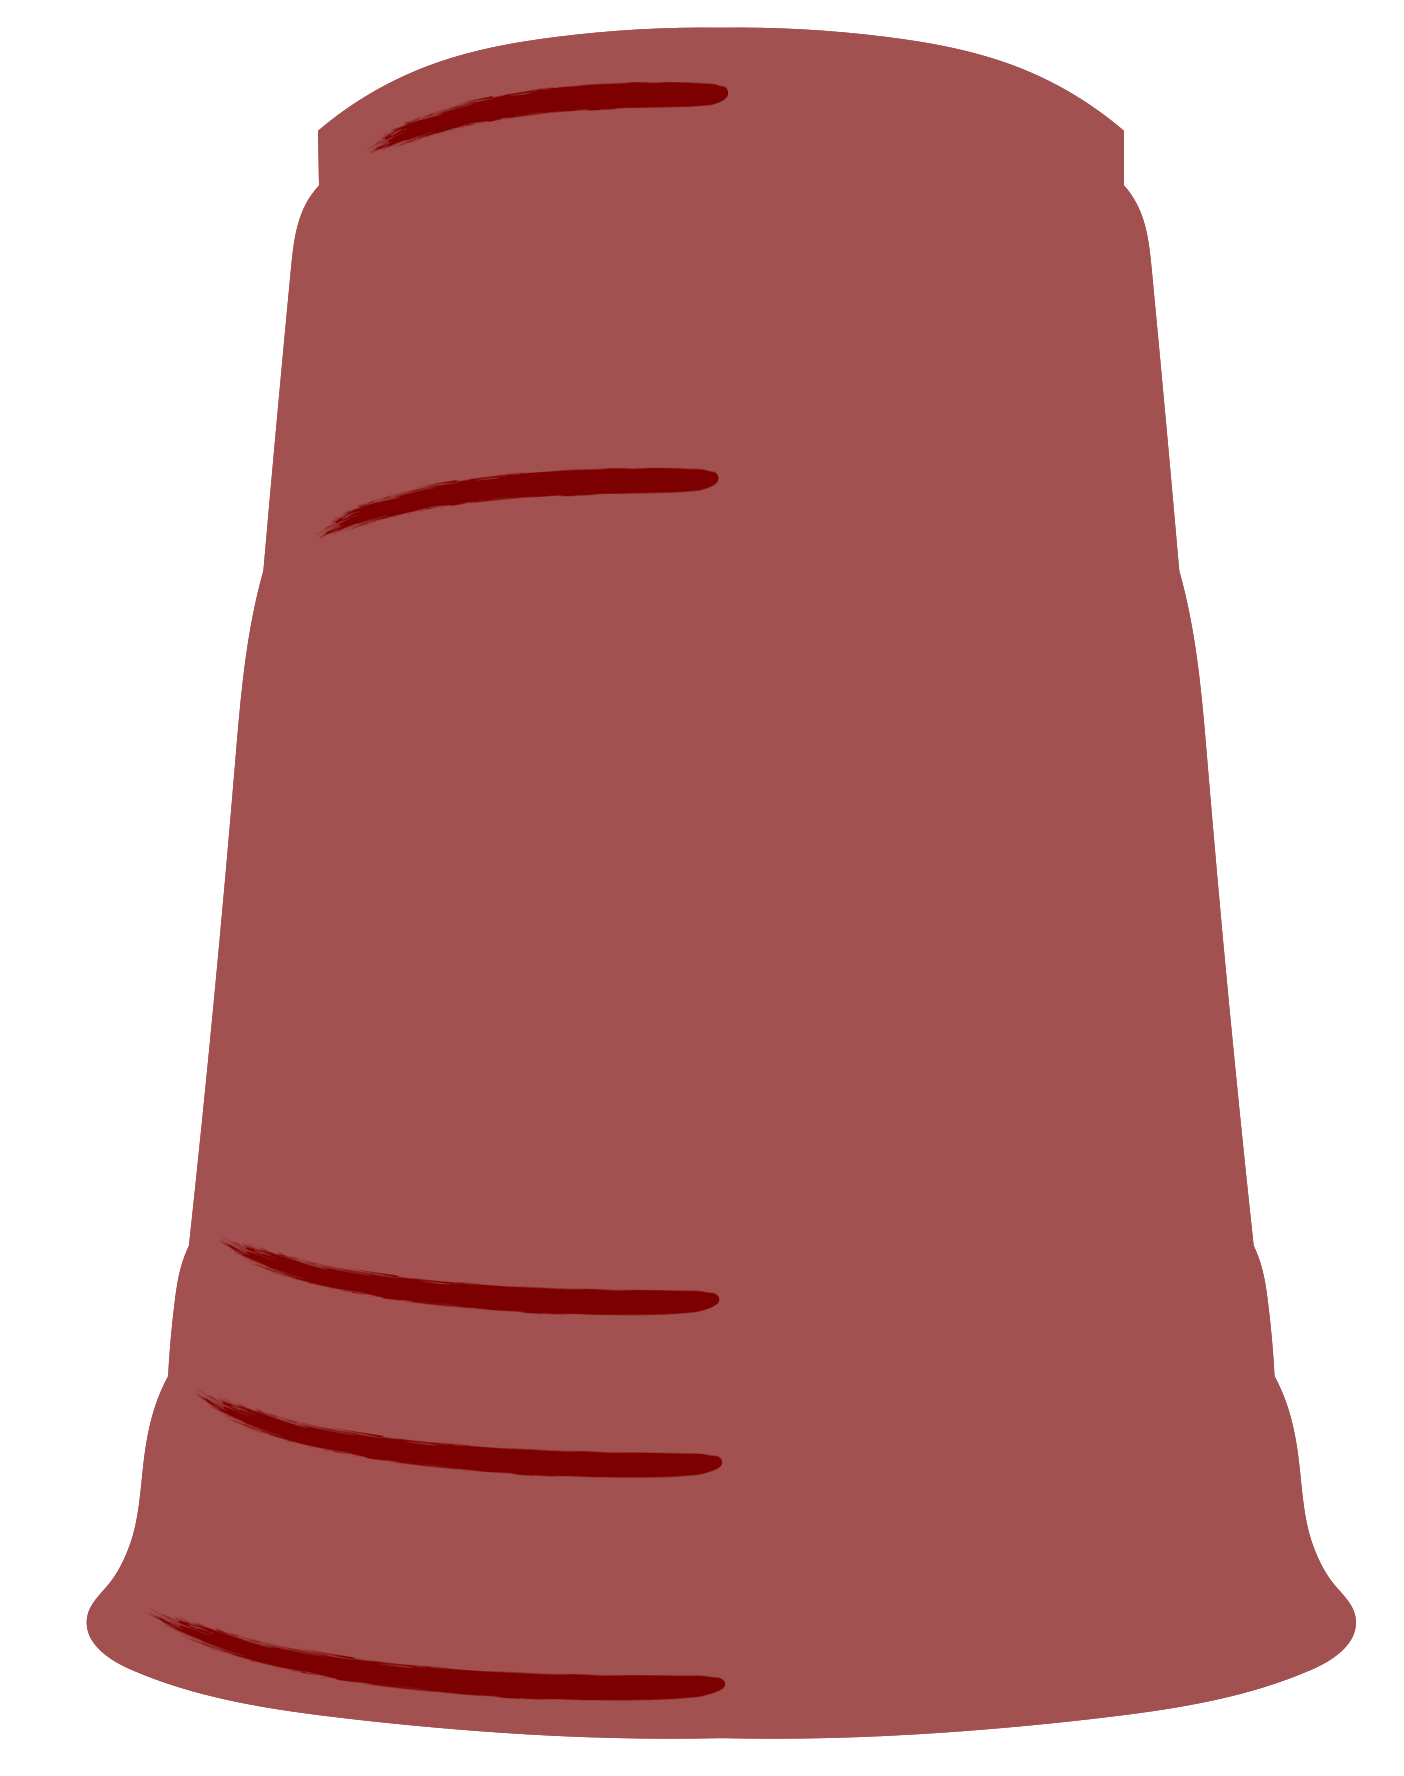
\includegraphics[width=2cm]{cup_down.png}};
  
\fill[dark] (0, 4) circle (1);
\node at (0, 7) {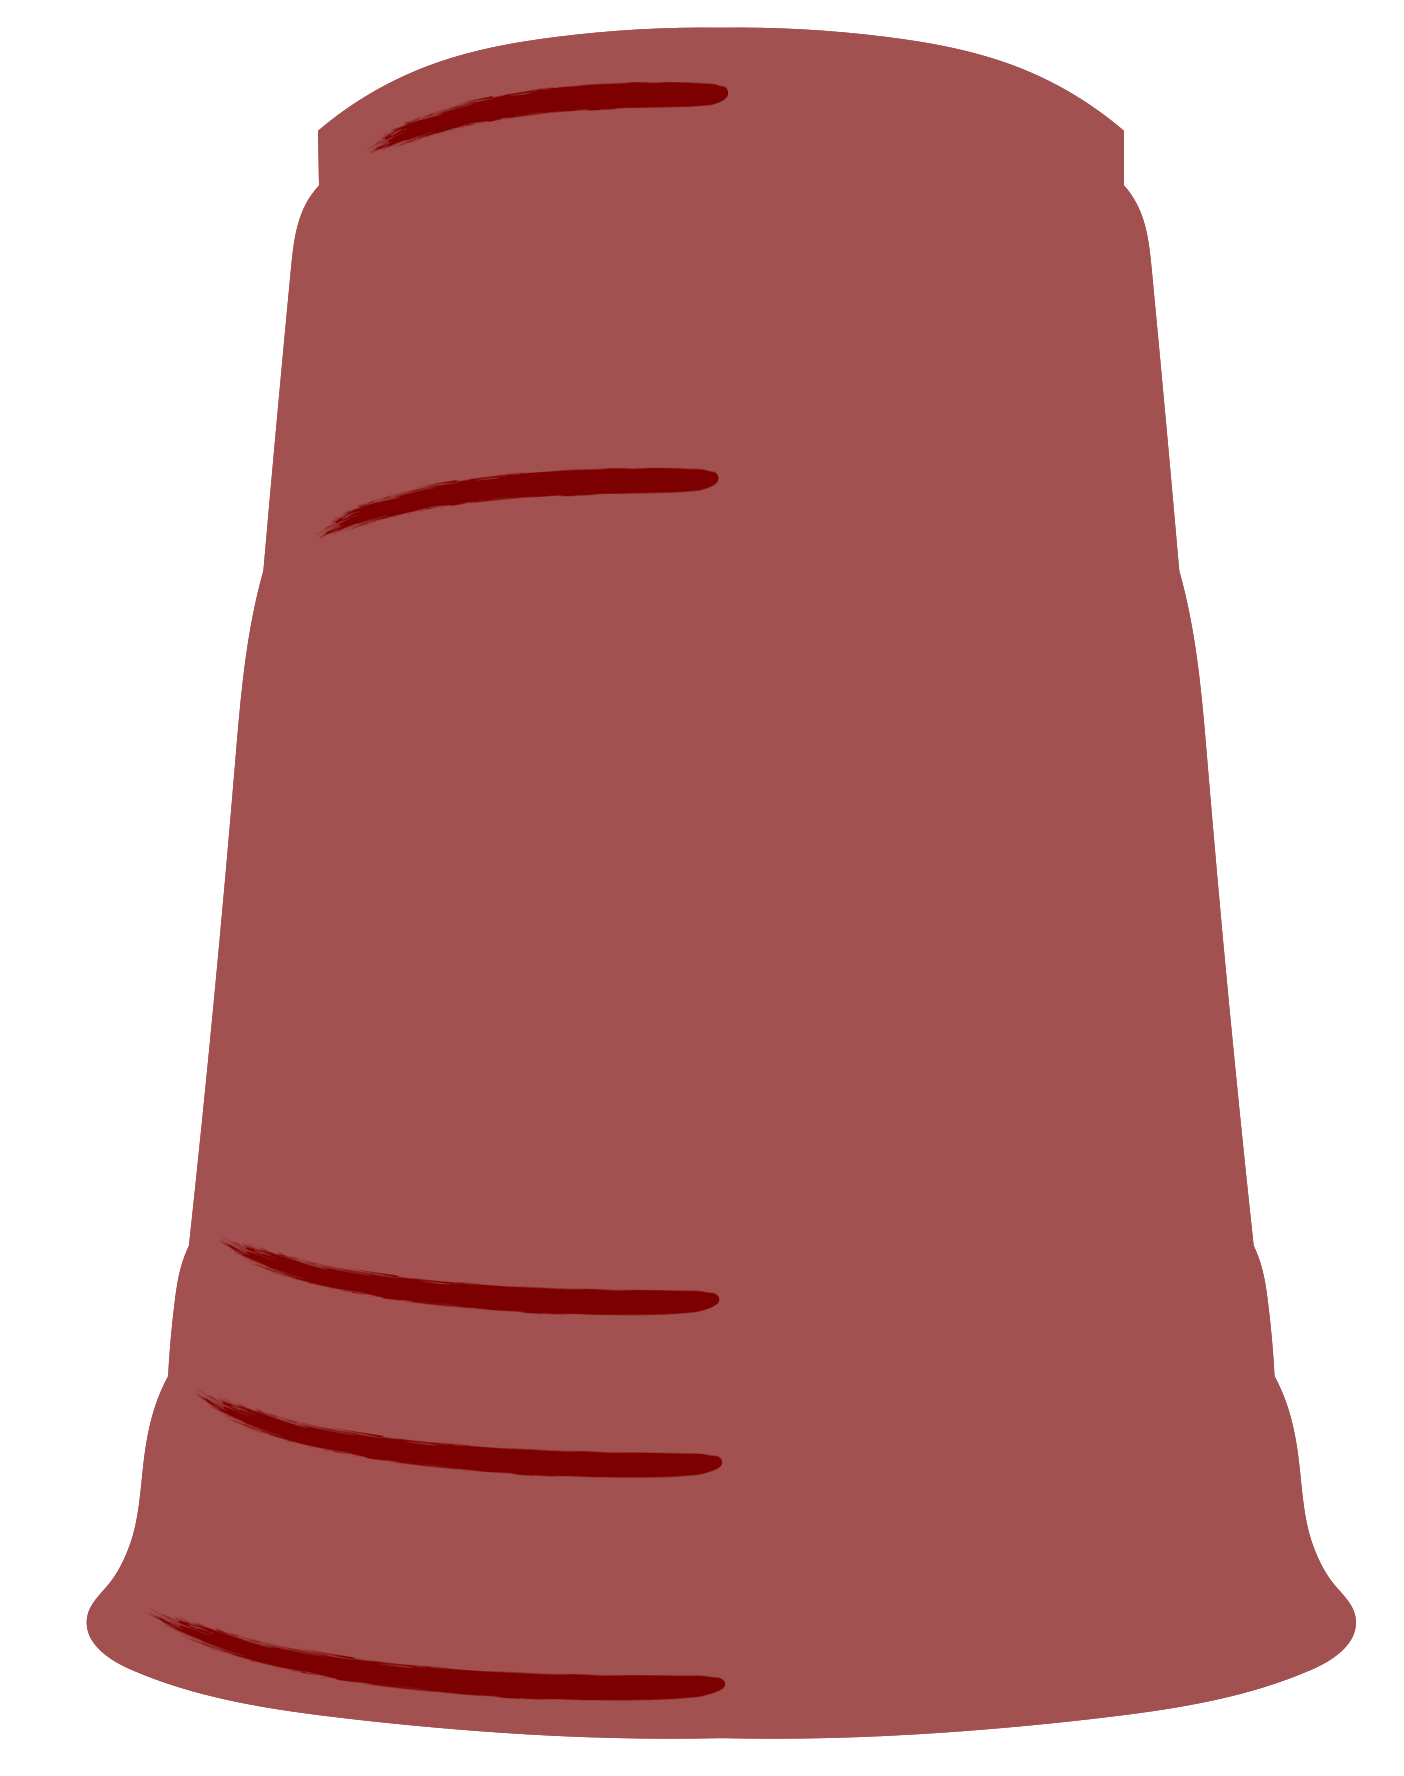
\includegraphics[width=2cm]{cup_down.png}};

\fill[dark] (+10, 4) circle (1);
\node at (+10, 7) {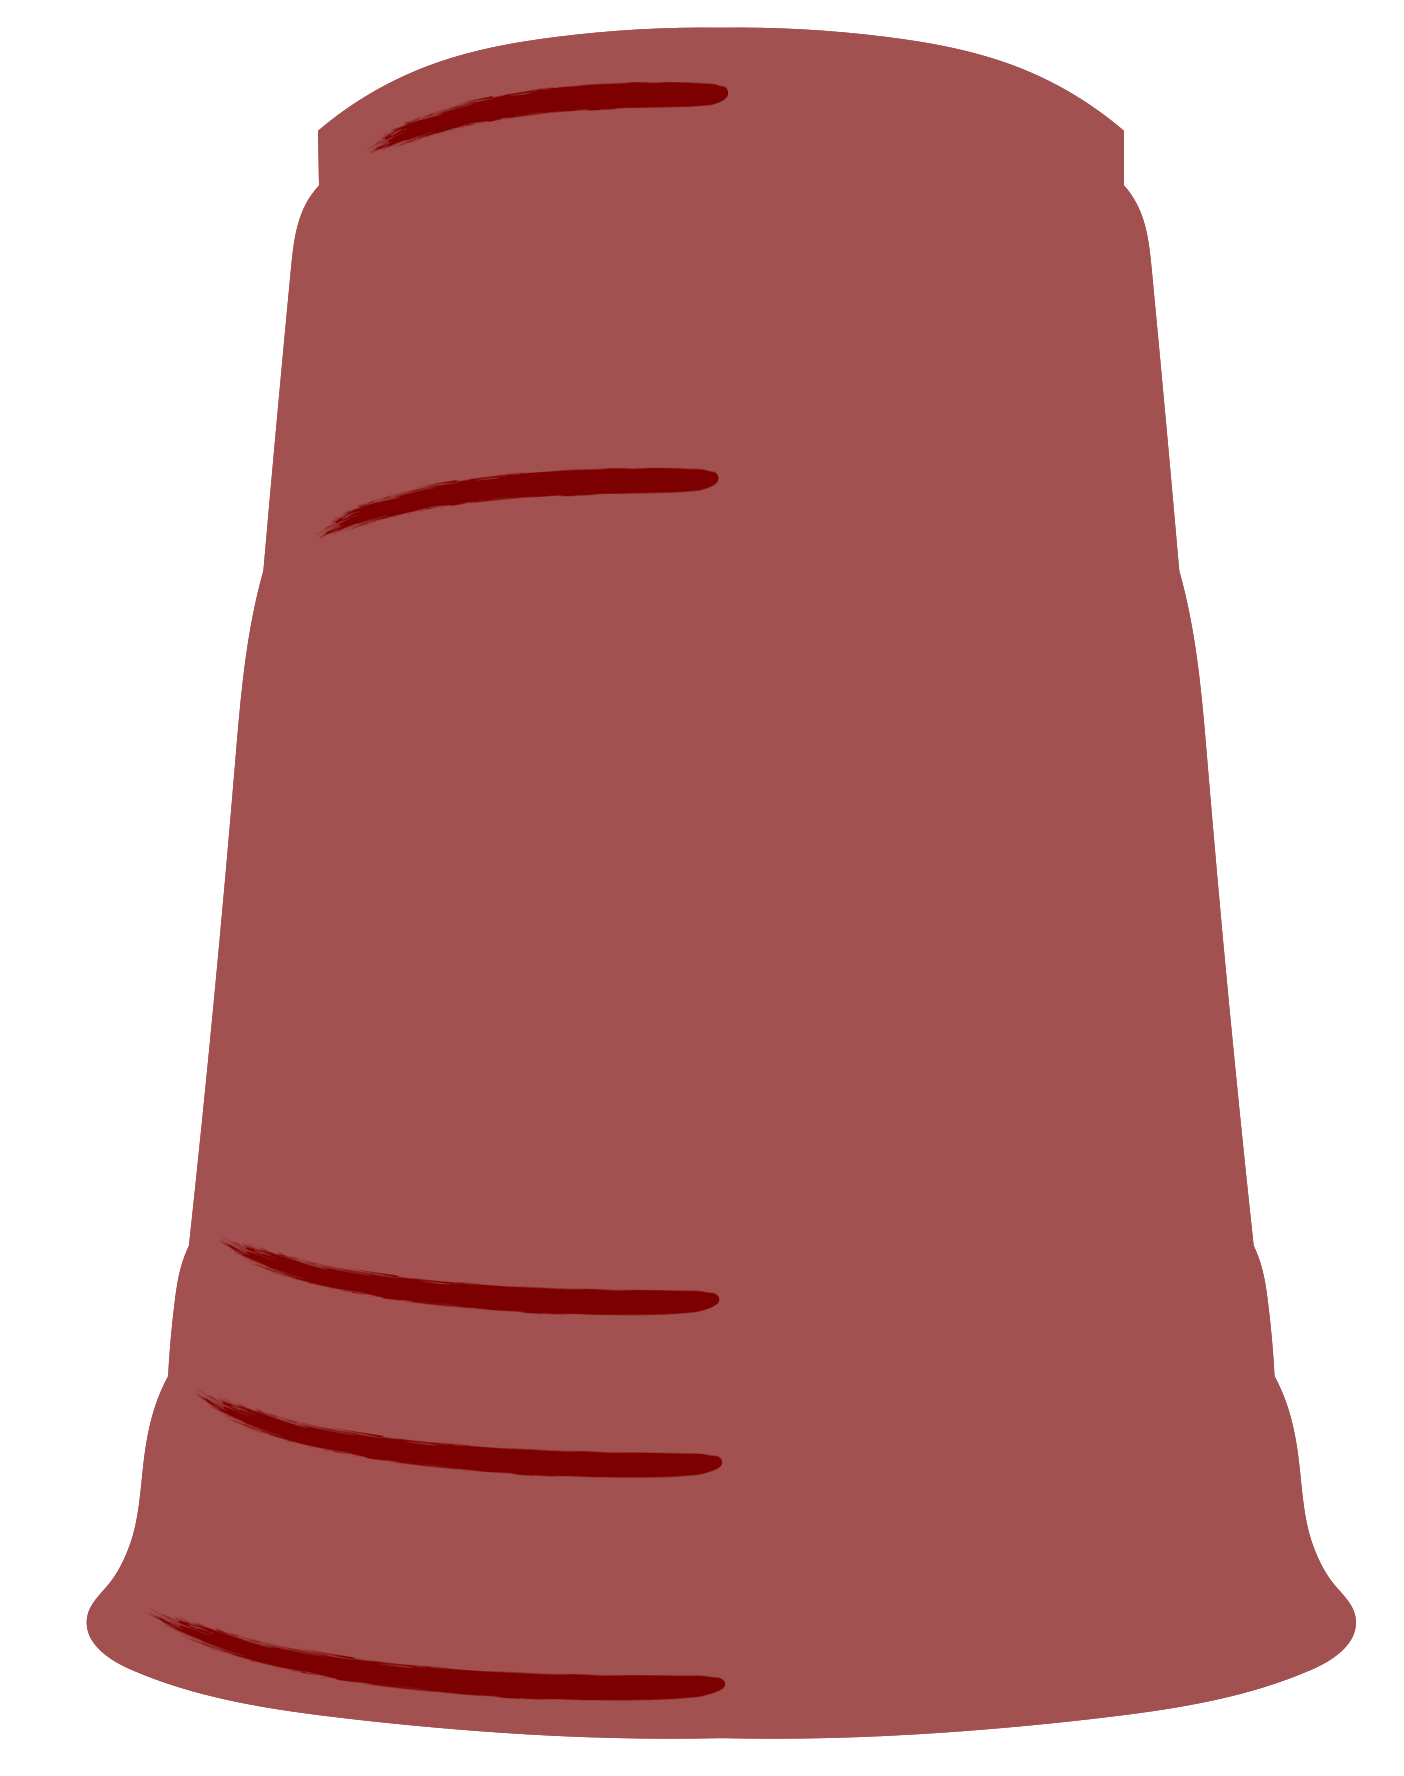
\includegraphics[width=2cm]{cup_down.png}};

\end{scope}

% Right
\begin{scope}[shift={(36, 0)}]

\draw[white] (-17, 0) rectangle (17, 15);

\fill[dark] (-10, 4) circle (1);
\node at (-10, 7) {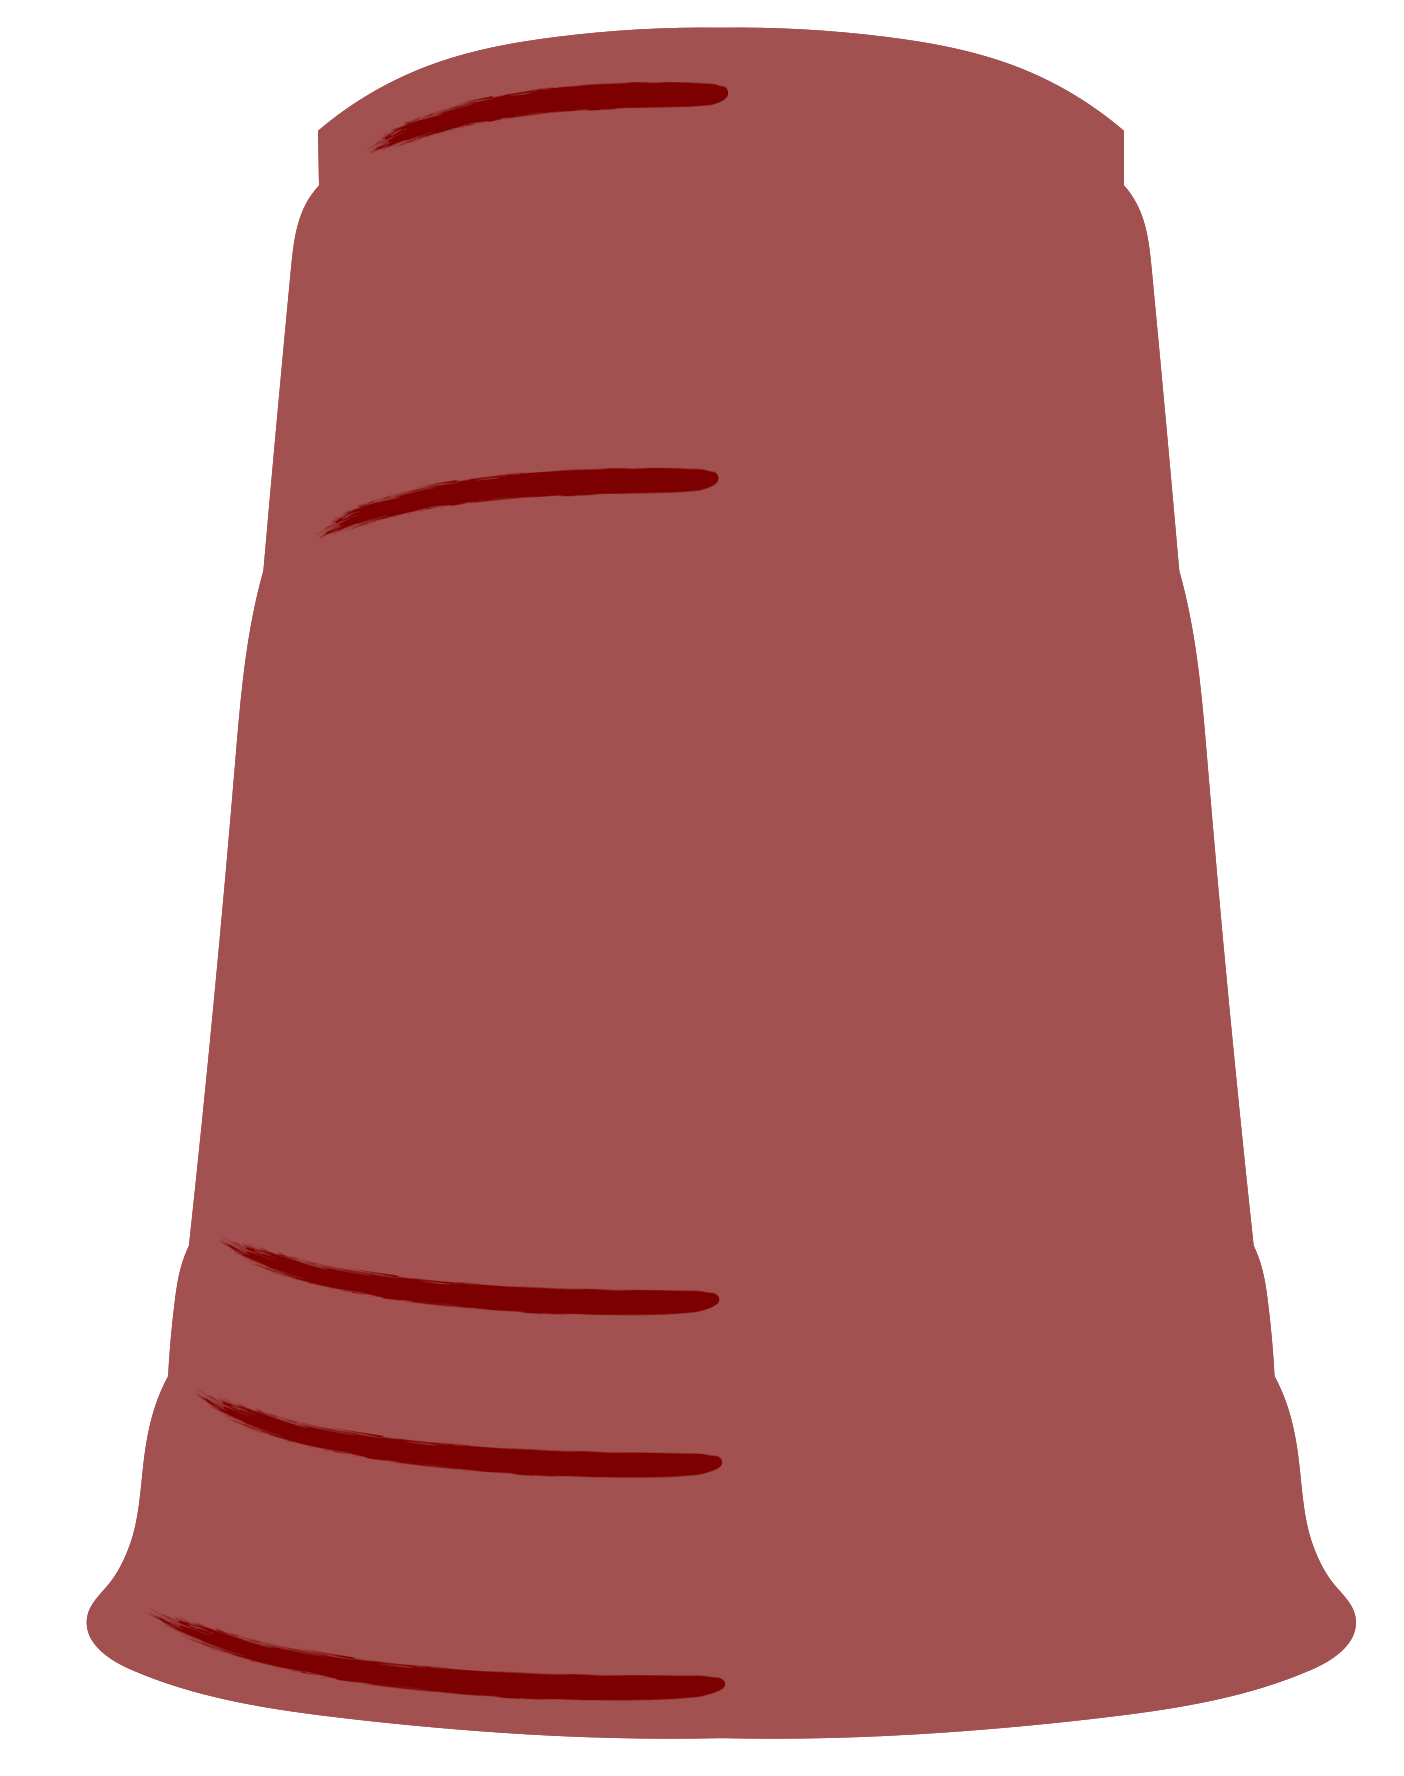
\includegraphics[width=2cm]{cup_down.png}};
  
\fill[dark] (0, 4) circle (1);
\node at (0, 7) {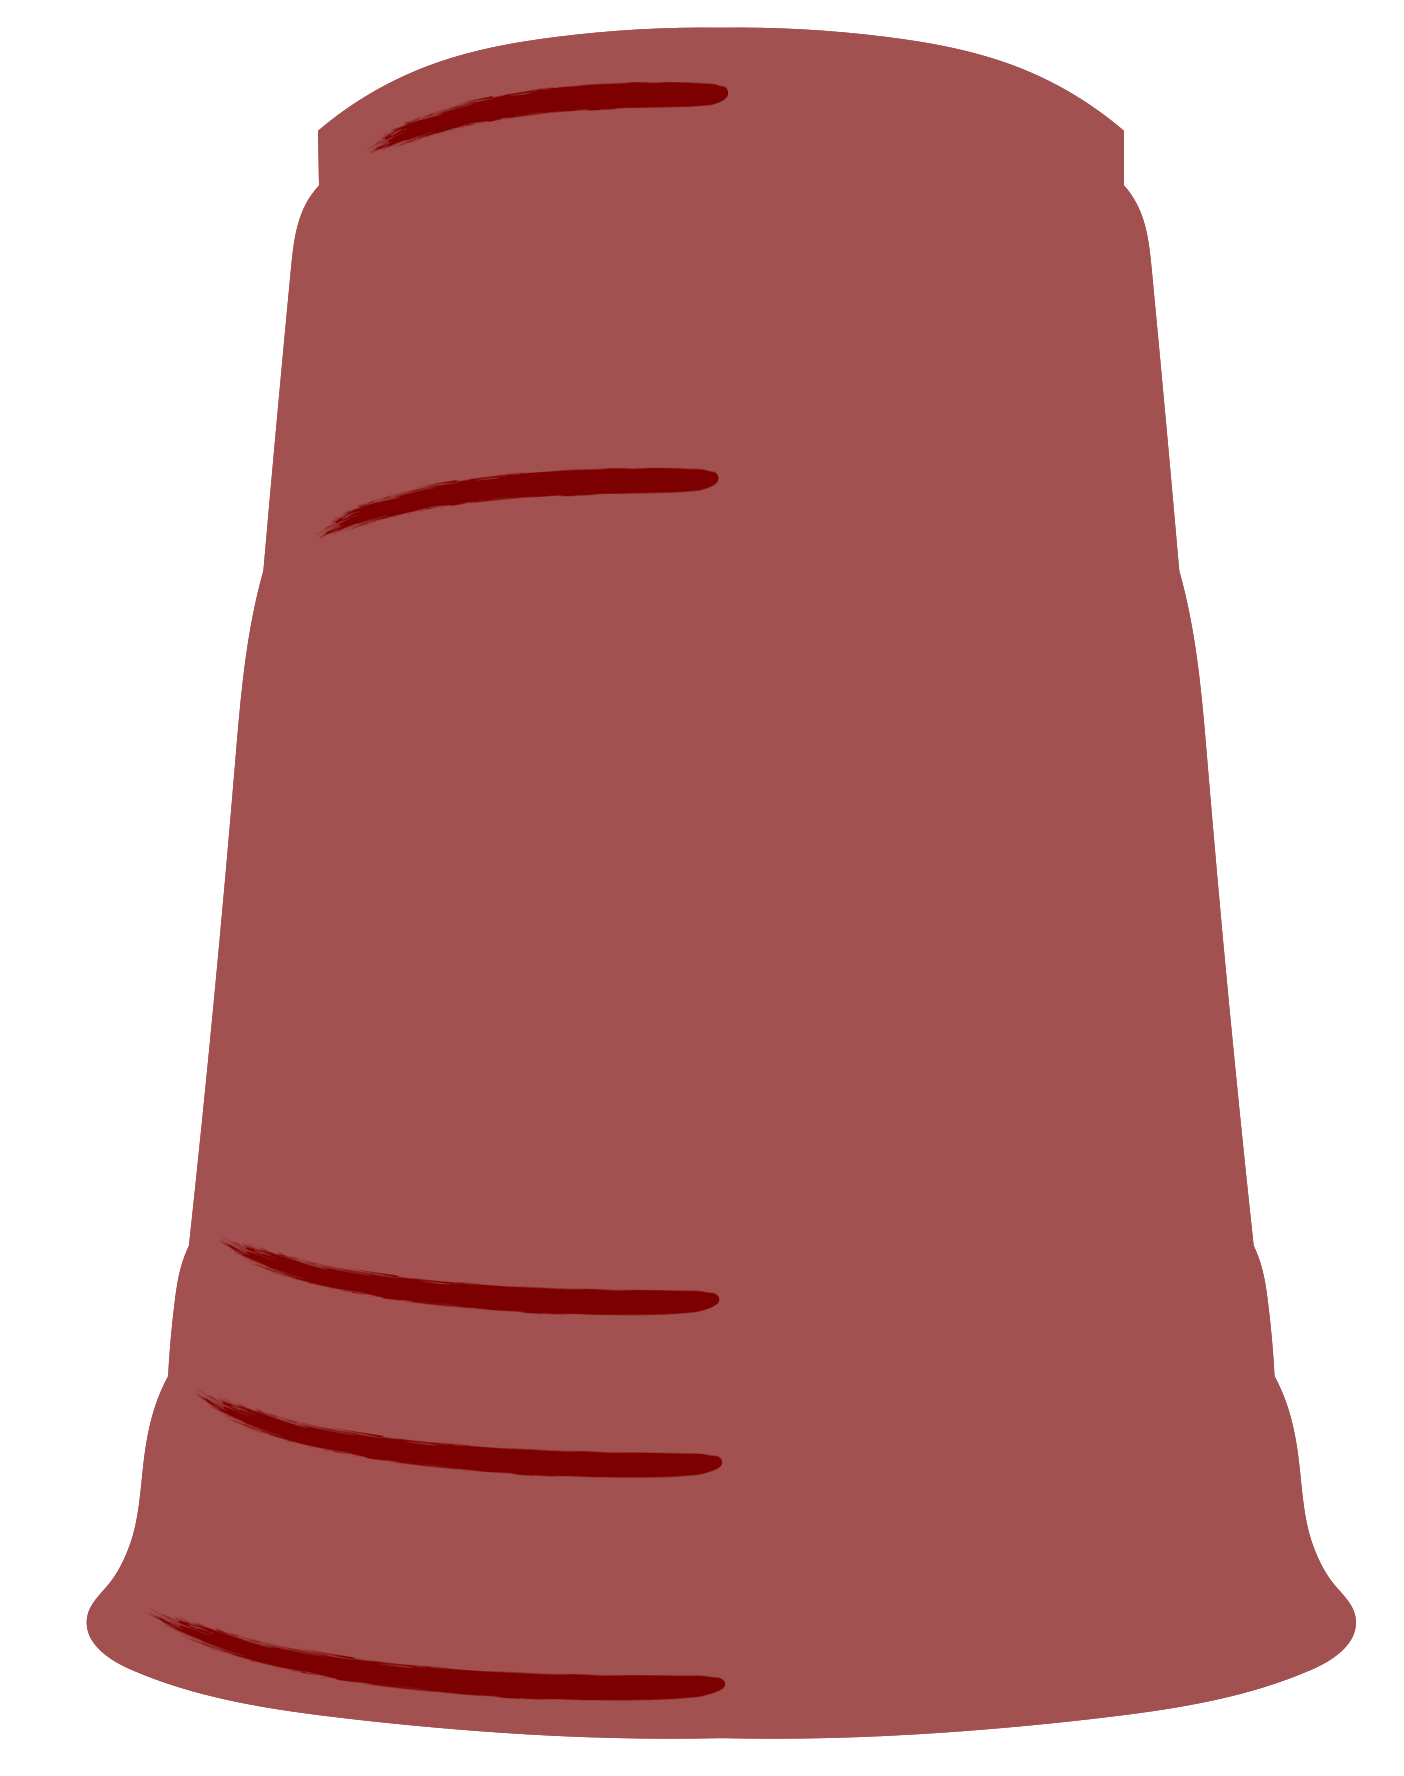
\includegraphics[width=2cm]{cup_down.png}};

\fill[dark] (+10, 4) circle (1);
\node at (+10, 7) {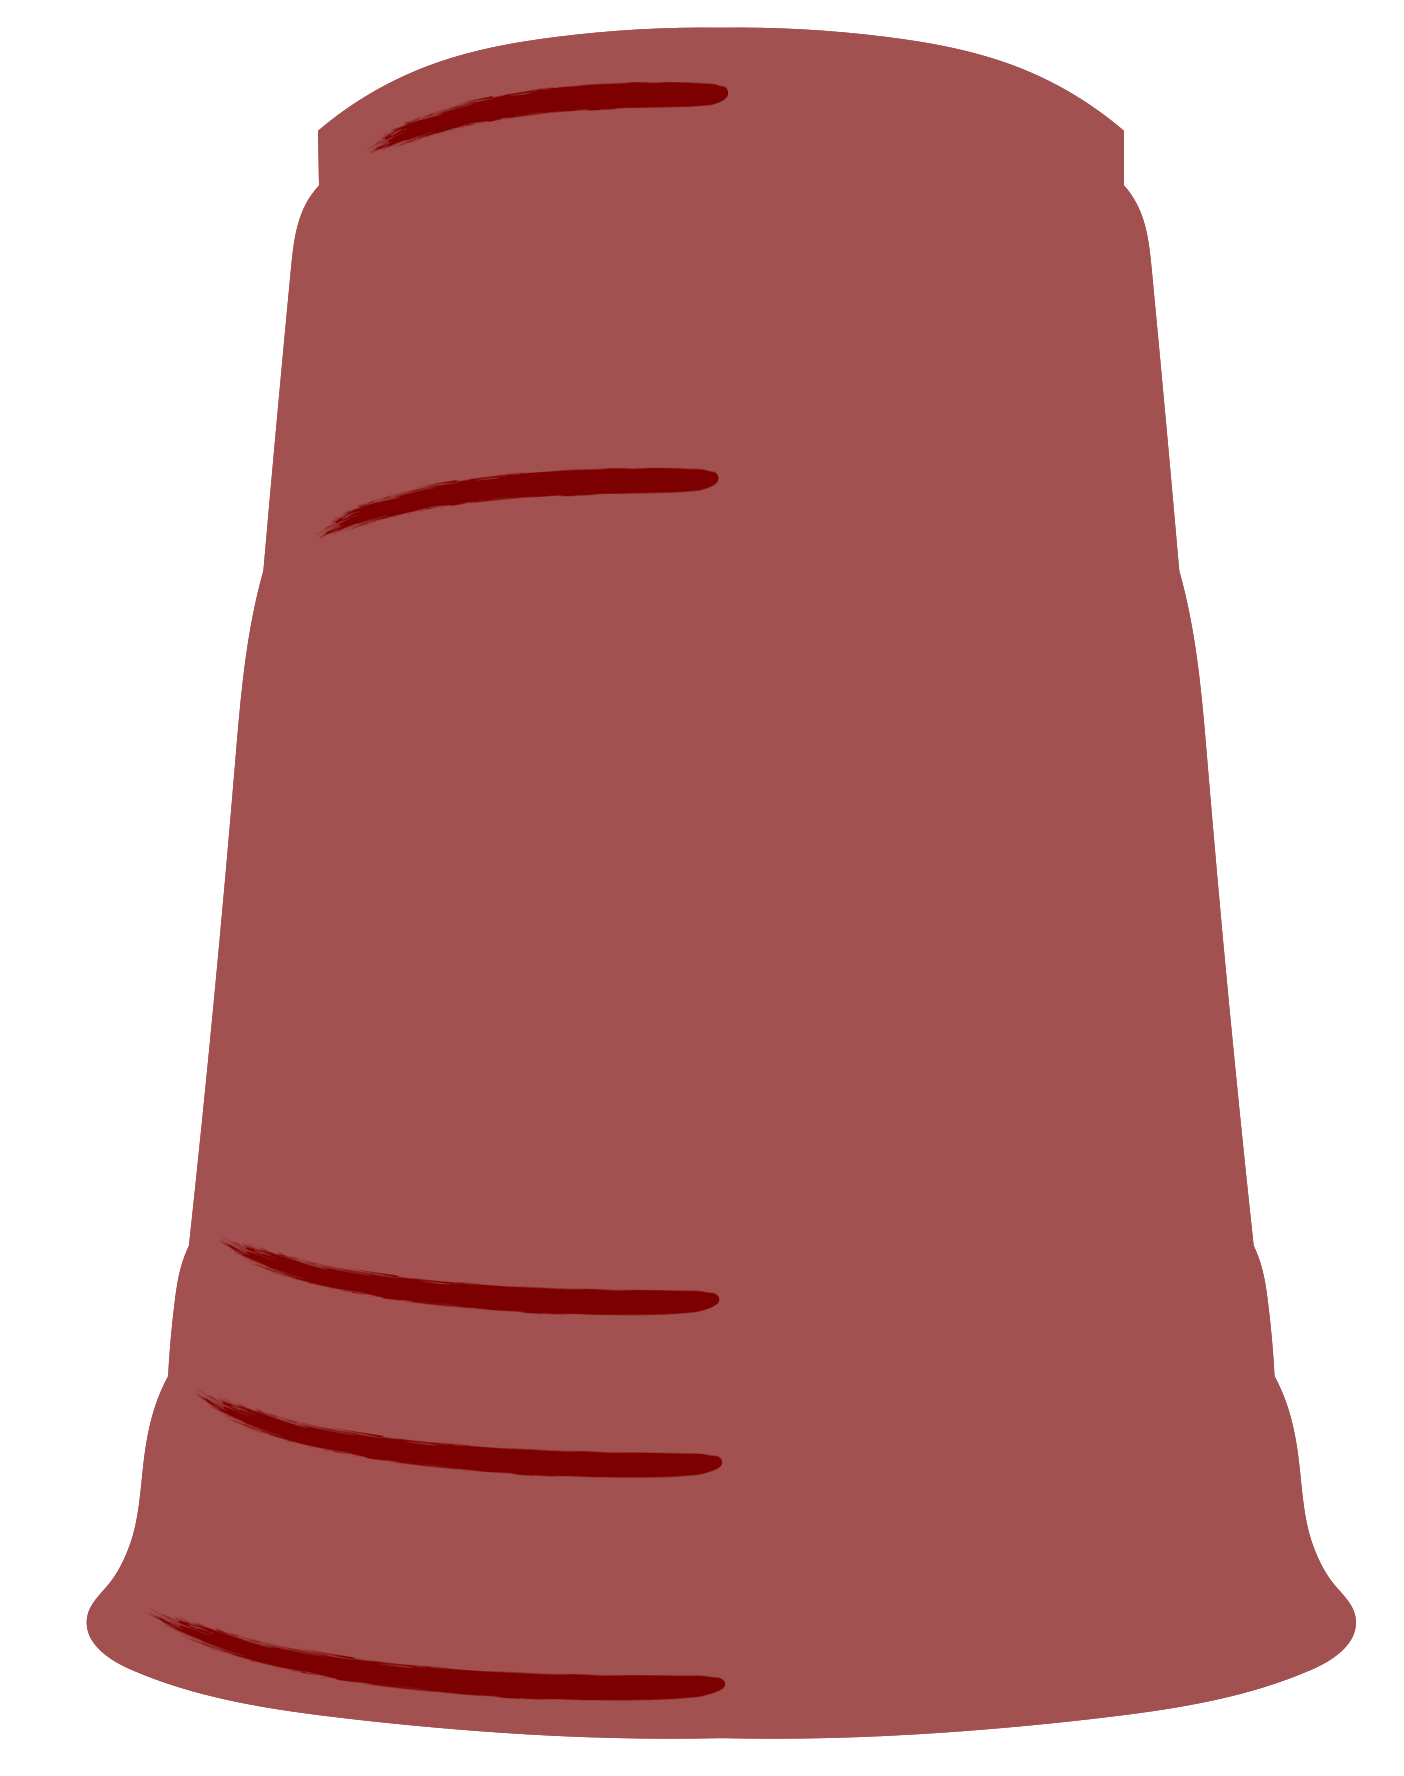
\includegraphics[width=2cm]{cup_down.png}};

\pgfmathsetmacro{\r}{10}
\pgfmathsetmacro{\start}{160}
\pgfmathsetmacro{\stop}{20}

\draw[dark, ->, >=stealth] ({0 + \r * cos(\start)}, {8 + \r * sin(\start)}) 
                arc[x radius = \r, y radius = 3, start angle=\start, end angle= \stop];

\pgfmathsetmacro{\r}{3}
\pgfmathsetmacro{\start}{160}
\pgfmathsetmacro{\stop}{20}

\draw[dark, ->, >=stealth] ({-5 + \r * cos(\start)}, {10 + \r * sin(\start)}) 
                arc[x radius = \r, y radius = 0.75, start angle=\start, end angle= \stop];

\draw[dark, ->, >=stealth] ({5 + \r * cos(\start)}, {10 + \r * sin(\start)}) 
                arc[x radius = \r, y radius = 0.75, start angle=\start, end angle= \stop];

\pgfmathsetmacro{\r}{10}
\pgfmathsetmacro{\start}{340}
\pgfmathsetmacro{\stop}{200}

\draw[dark, ->, >=stealth] ({0 + \r * cos(\start)}, {6 + \r * sin(\start)}) 
                arc[x radius = \r, y radius = 3, start angle=\start, end angle= \stop];

\pgfmathsetmacro{\r}{2}
\pgfmathsetmacro{\start}{340}
\pgfmathsetmacro{\stop}{200}

\draw[dark, ->, >=stealth] ({-5 + \r * cos(\start)}, {3.5 + \r * sin(\start)}) 
                arc[x radius = \r, y radius = 0.75, start angle=\start, end angle= \stop];

\draw[dark, ->, >=stealth] ({5 + \r * cos(\start)}, {3.5 + \r * sin(\start)}) 
                arc[x radius = \r, y radius = 0.75, start angle=\start, end angle= \stop];


\pgfmathsetmacro{\r}{1}
\pgfmathsetmacro{\start}{-160}
\pgfmathsetmacro{\stop}{140}

\draw[dark, ->, >=stealth] ({-6 + \r * cos(\start)}, {7 + \r * sin(\start)}) 
                arc[x radius = \r, y radius = 0.25, start angle=\start, end angle= \stop];

\draw[dark, ->, >=stealth] ({4 + \r * cos(\start)}, {7 + \r * sin(\start)}) 
                arc[x radius = \r, y radius = 0.25, start angle=\start, end angle= \stop];

\draw[dark, ->, >=stealth] ({14 + \r * cos(\start)}, {7 + \r * sin(\start)}) 
                arc[x radius = \r, y radius = 0.25, start angle=\start, end angle= \stop];

\end{scope}

\end{tikzpicture}

\end{document}  